%!TEX program = xelatex

\documentclass[compress]{beamer}
%--------------------------------------------------------------------------
% Common packages
%--------------------------------------------------------------------------

\definecolor{links}{HTML}{663000}
\hypersetup{colorlinks,linkcolor=,urlcolor=links}

\usepackage[english]{babel}
\usepackage{pgfpages} % required for notes on second screen
\usepackage{graphicx}

\usepackage{multicol}

\usepackage{tabularx,ragged2e}
\usepackage{booktabs}

\setlength{\emergencystretch}{3em}  % prevent overfull lines
\providecommand{\tightlist}{%
  \setlength{\itemsep}{0pt}\setlength{\parskip}{0pt}}


\usetheme{hri}

% Display the navigation bullet even without subsections
\usepackage{remreset}% tiny package containing just the \@removefromreset command
\makeatletter
\@removefromreset{subsection}{section}
\makeatother
\setcounter{subsection}{1}

\makeatletter
\let\beamer@writeslidentry@miniframeson=\beamer@writeslidentry
\def\beamer@writeslidentry@miniframesoff{%
  \expandafter\beamer@ifempty\expandafter{\beamer@framestartpage}{}% does not happen normally
  {%else
    % removed \addtocontents commands
    \clearpage\beamer@notesactions%
  }
}
\newcommand*{\miniframeson}{\let\beamer@writeslidentry=\beamer@writeslidentry@miniframeson}
\newcommand*{\miniframesoff}{\let\beamer@writeslidentry=\beamer@writeslidentry@miniframesoff}
\makeatother



\newcommand{\source}[2]{{\tiny\it Source: \href{#1}{#2}}}

\usepackage{tikz}
\usetikzlibrary{mindmap,backgrounds,positioning,calc,patterns}
\usepackage{pgfplots}
\pgfplotsset{compat=newest}
\usepackage{circuitikz}

\graphicspath{{figs/}}

\title{ROCO222 \newline Intro to Sensors and Actuators}
\subtitle{Electromagnetism \& DC motor -- Part 2}

\date{}
\author{Séverin Lemaignan}
\institute{Centre for Robotics and Neural Systems\\{\bf Plymouth University}}

\begin{document}


%%%%%%%%%%%%%%%%%%%%%%%%%%%%%%%%%%%%%%%%%%%%%%%%%%%%%%%%

\licenseframe{github.com/severin-lemaignan/module-introduction-sensors-actuators}

%%%%%%%%%%%%%%%%%%%%%%%%%%%%%%%%%%%%%%%%%%%%%%%%%%%%%%%%

\maketitle

%%%%%%%%%%%%%%%%%%%%%%%%%%%%%%%%%%%%%%%%%%%%%%%%%%%%%%%%

\section{DC motors datasheets}

{\fullbackground[scale=0.9,page=2]{ian-dc-motor-datasheet.pdf}
    \begin{frame}{Maxon DC motor variants}
    \end{frame}
}

{\fullbackground[scale=0.9,page=3]{ian-dc-motor-datasheet.pdf}
    \begin{frame}{Development of permanent magnets}
    \end{frame}
}

{\fullbackground[scale=0.9,page=4]{ian-dc-motor-datasheet.pdf}
    \begin{frame}{Permanent magnets}
    \end{frame}
}

{\fullbackground[scale=0.9,page=5]{ian-dc-motor-datasheet.pdf}
    \begin{frame}{Understanding motor datasheets}
    \end{frame}
}

{\fullbackground[scale=0.9,page=6]{ian-dc-motor-datasheet.pdf}
    \begin{frame}{DC motor data}
    \end{frame}
}

{\fullbackground[scale=0.9,page=7]{ian-dc-motor-datasheet.pdf}
    \begin{frame}{Speed-voltage characteristic}
    \end{frame}
}

{\fullbackground[scale=0.9,page=8]{ian-dc-motor-datasheet.pdf}
    \begin{frame}{Speed-torque characteristic}
    \end{frame}
}

{\fullbackground[scale=0.9,page=9]{ian-dc-motor-datasheet.pdf}
    \begin{frame}{Motor values at nominal voltage}
    \end{frame}
}

{\fullbackground[scale=0.9,page=10]{ian-dc-motor-datasheet.pdf}
    \begin{frame}{Operating points}
    \end{frame}
}

{\fullbackground[scale=0.9,page=11]{ian-dc-motor-datasheet.pdf}
    \begin{frame}{Effect of changing the windings}
    \end{frame}
}

{\fullbackground[scale=0.9,page=12]{ian-dc-motor-datasheet.pdf}
    \begin{frame}{Torque constant $K_M$}
    \end{frame}
}

{\fullbackground[scale=0.9,page=13]{ian-dc-motor-datasheet.pdf}
    \begin{frame}{Torque constant $K_M$}
    \end{frame}
}

{\fullbackground[scale=0.9,page=14]{ian-dc-motor-datasheet.pdf}
    \begin{frame}{Speed constant $K_n$}
    \end{frame}
}

{\fullbackground[scale=0.9,page=15]{ian-dc-motor-datasheet.pdf}
    \begin{frame}{Nominal motor characteristics}
    \end{frame}
}

{\fullbackground[scale=0.9,page=16]{ian-dc-motor-datasheet.pdf}
    \begin{frame}{List of main motor parameters}
    \end{frame}
}

{\fullbackground[scale=0.9,page=17]{ian-dc-motor-datasheet.pdf}
    \begin{frame}{Motor thermal considerations}
    \end{frame}
}

{\fullbackground[scale=0.9,page=18]{ian-dc-motor-datasheet.pdf}
    \begin{frame}{Influence of temperature on motor operation}
    \end{frame}
}

{\fullbackground[scale=0.9,page=19]{ian-dc-motor-datasheet.pdf}
    \begin{frame}{Nominal torque and temperature}
    \end{frame}
}

{\fullbackground[scale=0.9,page=20]{ian-dc-motor-datasheet.pdf}
    \begin{frame}{Motor limits: operation ranges}
    \end{frame}
}

{\fullbackground[scale=0.9,page=21]{ian-dc-motor-datasheet.pdf}
    \begin{frame}{Short-term overload operation}
    \end{frame}
}

{\fullbackground[scale=0.9,page=22]{ian-dc-motor-datasheet.pdf}
    \begin{frame}{List of main thermal motor parameters}
    \end{frame}
}

{\fullbackground[scale=0.9,page=23]{ian-dc-motor-datasheet.pdf}
    \begin{frame}{List of main mechanical motor parameters}
    \end{frame}
}

{\fullbackground[scale=0.9,page=24]{ian-dc-motor-datasheet.pdf}
    \begin{frame}{List of main mechanical motor parameters}
    \end{frame}
}

{\fullbackground[scale=0.9,page=25]{ian-dc-motor-datasheet.pdf}
    \begin{frame}{Other specifications}
    \end{frame}
}


{\fullbackground[scale=0.9,page=26]{ian-dc-motor-datasheet.pdf}
    \begin{frame}{Motor size selection}
    \end{frame}
}


\miniframesoff
\begin{frame}[plain]
    \begin{center}
        \Large
        10 min break\\[2em]
    \end{center}
\end{frame}
\miniframeson

\section[Recap]{So far in electromagnetism...}

\begin{frame}{Recap of last lecture}
    \begin{itemize}
        \item Ampère's law
        \item Faraday's law of induction: $\displaystyle\mathcal{E} = -N \cdot \frac{d\Phi_B}{dt}$
        \item Lenz law
        \item Lorentz law
    \end{itemize}
\end{frame}

\section{Inductance}

{\fullbackground[scale=0.9,page=39]{ian-electromagnetism.pdf}
    \begin{frame}{Electrical resistance}
    \end{frame}
}

{\fullbackground[scale=0.9,page=40]{ian-electromagnetism.pdf}
    \begin{frame}{Electrical inductance}
    \end{frame}
}

{\fullbackground[scale=0.9,page=41]{ian-electromagnetism.pdf}
    \begin{frame}{Current in an LR circuit}
    \end{frame}
}

{\fullbackground[scale=0.9,page=42]{ian-electromagnetism.pdf}
    \begin{frame}{Current in an LR circuit}
    \end{frame}
}

{\fullbackground[scale=0.9,page=43]{ian-electromagnetism.pdf}
    \begin{frame}{Definition of inductance}
    \end{frame}
}

{\fullbackground[scale=0.9,page=44]{ian-electromagnetism.pdf}
    \begin{frame}{Inductance of a solenoid}
    \end{frame}
}


\begin{frame}{Consequence for motors}

    \only<1>{
  Moving a magnet in a coil induces current:


    \begin{center}
        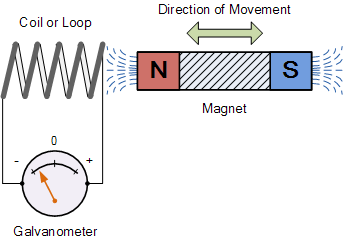
\includegraphics[width=0.6\linewidth]{image29}

    \scalebox{1.5}{Faraday's law of induction: $\displaystyle\mathcal{E} = - \cdot \frac{d\Phi_B}{dt}$}

    \end{center}
}

    \only<2>{
        
    If a coil consists of N loops with the same area, the total induced EMF in
    the coil is given by:

\[
        \mathcal{E} = -N \cdot \frac{d\Phi_B}{dt}
\]

In a uniform magnetic field, the induced EMF can be expressed as:

\[
    \mathcal{E} = -N \cdot \frac{d}{dt} (B A cos(\theta)) = - N \cdot B \cdot A \frac{d cos(\theta)}{dt} = -N \cdot B \cdot A \cdot sin(\theta) \cdot \dot\theta
\]

With enough coils,

\[
    \mathcal{E} = - N \cdot B \cdot A \cdot \dot\theta = K_e \dot\theta
\]

    $K_e$ is the \textbf{back-EMF} constant of the motor.


    }
\end{frame}

\begin{frame}{Electrical generator}

    \begin{center}
        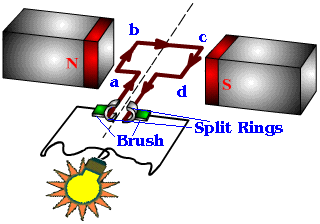
\includegraphics[width=0.6\linewidth]{image30}
    \end{center}

\begin{itemize}

\item Speed of rotation affects voltage generated
\item So how fast will a motor rotate with applied voltage $V$?
\item Lets consider the equivalent circuit for a DC motor
\end{itemize}
\end{frame}

\begin{frame}{DC motor equivalent circuit}

    \begin{center}
        \resizebox{0.6\linewidth}{!}{
            % Based on http://texample.net/tikz/examples/induction-machine/
            \begin{circuitikz}
                \draw
                % rotor circuit
                (0,0) to [short, *-] (6,0)
                to [V, l_={EMF}] (6,2) % rotor emf

                % stator circuit
                (0,0) to [open, v^>=$V$] (0,2) % stator voltage
                to [short, *- ,i=$I$] (1,2) % stator current
                to [R, l=$R$] (3,2) % stator resistance
                to [L, l=$L$] (6,2); % leakage inductance
            \end{circuitikz}
        }
    \end{center}

\footnotesize
\begin{itemize}

\item $V$ is the applied voltage, $I$ is the drawn current
\item Resistance $R$ arises from the coil and the brushes
\item Inductance $L$ arises from the coil
\item Back EMF arises from rotation of the coil in the magnetic field
  created by the stator magnets
\end{itemize}

\end{frame}

\begin{frame}{Voltage in a DC motor}

    \begin{center}
        \resizebox{0.6\linewidth}{!}{
            % Based on http://texample.net/tikz/examples/induction-machine/
            \begin{circuitikz}
                \draw
                % rotor circuit
                (0,0) to [short, *-] (6,0)
                to [V, l_={EMF $\mathcal{E}$}] (6,2) % rotor emf

                % stator circuit
                (0,0) to [open, v^>=$V$] (0,2) % stator voltage
                to [short, *- ,i=$I$] (1,2) % stator current
                to [R, l=$R$] (3,2) % stator resistance
                to [L, l=$L$] (6,2); % leakage inductance
            \end{circuitikz}
        }
    \end{center}

\textbf{Kirchhoff's voltage law}: voltage across resistor, inductance and
back EMF balance applied voltage

\begin{align*}
    V &= I \cdot R + L \cdot \frac{dI}{dt} + \mathcal{E} \\
      &= I \cdot R + L \cdot \frac{dI}{dt} + K_e \cdot \dot\theta
\end{align*}

\pause

How to know $I$?

\end{frame}


\begin{frame}{Conservation of energy!}


    \textbf{Conservation of energy means electrical power in = mechanical power out +
    losses}



    \begin{columns}
        \begin{column}{0.7\linewidth}
    \begin{center}
        \resizebox{0.9\linewidth}{!}{
            \begin{tikzpicture}[>=latex]

                \node at (0,0) (motor) {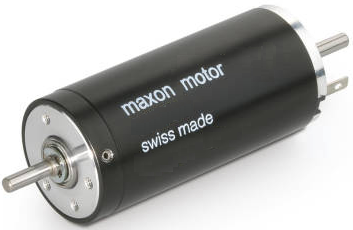
\includegraphics[width=3cm]{../part2/figs/maxon}};
                \node[below left=0.5 of motor] (pmech) {$P_{mech}= \tau \cdot \dot\theta$};
                \node[above right=0.5 of motor] (pel) {$P_{el}= V \cdot I$};
                \node[below right=0.5 of motor] (pr) {$P_{r}=R \cdot I^2$};
                \draw[ultra thick, red,->] (motor) -- (pmech);
                \draw[ultra thick, red,->] (pel) -- (motor);
                \draw[ultra thick, orange,->] (motor) -- (pr);
            \end{tikzpicture}
        }

    \end{center}

        \end{column}
        \begin{column}{0.3\linewidth}
    \footnotesize
    where:

        $\tau$ = torque;
        
        $\dot\theta$ = angular velocity;
        
        $I$ = input current;
        
        $V$ = applied voltage;

        $R$ = windings resistance
            
        \end{column}
    \end{columns}

        \begin{center}
    \[
        P_{el} = P_{mech} + P_{r}
    \]
        \end{center}

\end{frame}


\begin{frame}{Remember torque}

\only<1>{
    \begin{center}
        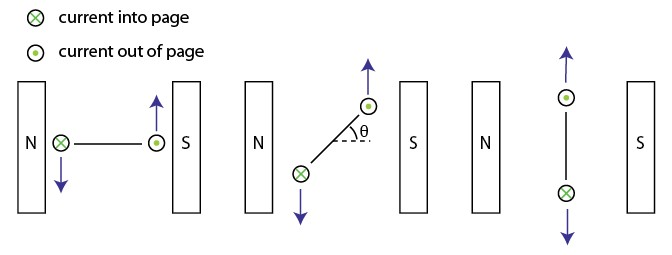
\includegraphics[width=0.8\linewidth]{../part2/figs/image16-3}
    \end{center}

If current $I$ flows through a coil of depth $L$ and width $d$ with $n$ turns,
    with magnetic field $B$, the coil pivots and generates a torque $\tau$ given
    by:

\[
\tau = n \cdot 2 (\frac{d}{2}) \cdot F \cdot cos(\theta) = n \cdot d \cdot B \cdot I \cdot L \cdot cos(\theta)
\]
}

    \only<2>{
With enough coils, we can remove the $cos(\theta)$ term:
\[
\tau = n \cdot d \cdot B \cdot I \cdot L = K_\tau \cdot I
\]


$K_\tau$ is the motor's torque constant.

}

\end{frame}

\begin{frame}{Putting it all together}

    \begin{columns}
        \begin{column}{0.5\linewidth}

    \begin{itemize}
        \item $V = K_e \cdot \dot\theta + I \cdot R$
        \item $\tau = K_\tau \cdot I$

    \end{itemize}
        \end{column}
        \begin{column}{0.5\linewidth}
    $V$ = applied voltage
            
    $\dot\theta$ = motor angular velocity
            
    $I$ = motor current
    
    $R$ = motor resistance
    
    $\tau$ = torque, including frictional losses
        \end{column}
    \end{columns}


    \pause 

    \begin{itemize}
        \item Electrical power in: $V \cdot I = K_e \cdot \dot\theta \cdot I + I^2 \cdot R$
        \item Mechanical power out: $\tau \cdot \dot\theta = K_\tau \cdot I \cdot \dot\theta$
        \item Losses: $I^2 \cdot R$
    \end{itemize}

    \pause

    Conservation of energy means electrical power in = mechanical power out +
    losses.

    This is true if and only if $K_e=K_\tau$.

    \pause

    \textbf{In a DC motor, the torque constant and back-EMF constants are equal.}
\end{frame}

\begin{frame}{Back to the voltage}


\begin{align*}
    V &= K_e \cdot \dot\theta + I \cdot R \\
    \tau &= K_\tau \cdot I \Rightarrow I = \frac{\tau}{k_\tau}
\end{align*}

\begin{equation*}
\begin{split}
    \Rightarrow V &= \frac{\tau}{K_\tau} \cdot R + K_e \cdot \dot\theta \\
    \Rightarrow \dot\theta &= \frac{V}{K} - \frac{\tau}{K^2} \cdot R
\end{split}
\end{equation*}

\end{frame}


\begin{frame}{How to choose the motor constants?}

    Rule of thumb with DC motor selection (also true for brushless DC motors to
    a large extent) -- pick a motor with a $K_T$ and back-EMF constant such that
    the supply voltage you have available is well-matched with the back-emf at
    your maximum speed. You usually want back-emf voltage to be 80-95\% of the
    supply voltage, but the exact number depends on the load torque and the $I R$
    drop in the motor at that operating point.

    If you pick a $K_T=K_e$ too high, you'll run out of voltage and won't be
    able to achieve the speed you need. If you pick a $K_T=K_e$ too low, the
    current needed to achieve the torque you need will be higher than necessary.

    \source{https://electronics.stackexchange.com/questions/33315/understanding-motor-constants-kt-and-kemf-for-comparing-brushless-dc-motors}{stackexchange}
\end{frame}

%%%%%%%%%%%%%%%%%%%%%%%%%%%%%%%%%%%%%%%%%%%%%%%%%%%%%%%%%%%%%%%%%%%%%%%%%%%%%%%%%%%%%%%5
%%%%%%%%%%%%%%%%%%%%%%%%%%%%%%%%%%%%%%%%%%%%%%%%%%%%%%%%%%%%%%%%%%%%%%%%%%%%%%%%%%%%%%%5
%%%%%%%%%%%%%%%%%%%%%%%%%%%%%%%%%%%%%%%%%%%%%%%%%%%%%%%%%%%%%%%%%%%%%%%%%%%%%%%%%%%%%%%5

\section[Diff. equations]{Differential equation of DC motor rotation}

{\fullbackground[scale=0.9,page=6]{ian-simple-newtonian-mechanics.pdf}
\begin{frame}{Moment of Inertia}
%
%Resists with opposing torque proportional to angular acceleration
%
%    \begin{columns}
%        \begin{column}{0.5\linewidth}
%            \begin{center}
%                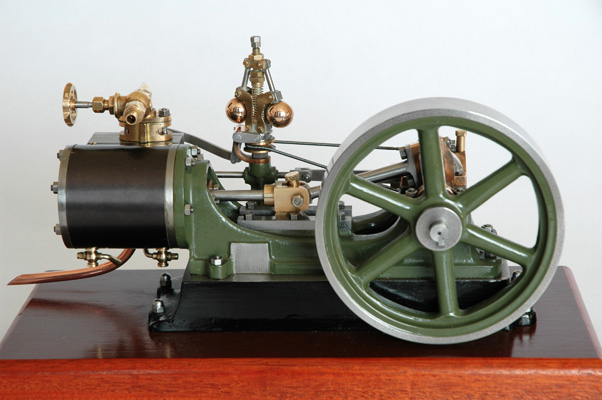
\includegraphics[height=0.3\paperheight]{image62}
%            \end{center}
%        \end{column}
%        \begin{column}{0.5\linewidth}
%            TBD
%        \end{column}
%    \end{columns}
%where
%
%$T$ is torque in $N\cdot m$
%
%$J$ is moment of inertial in $kg \cdot m^2$
%
\end{frame}
}

\begin{frame}{DC motor dynamics}

    \begin{center}
        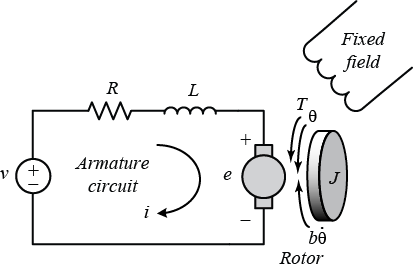
\includegraphics[width=0.5\linewidth]{image63}
    \end{center}

\only<1> {
\begin{itemize}

\item $R$ = Armature resistance (in ohms $\Omega$)
\item $L$ = Armature inductance (in Henrys $H$) % CHECK
\item $J$ = Moment of inertia for the motor rotor ($kg\cdot m^2$)
\item $b$ = Motor viscous friction constant (in $N\cdot m\cdot s$)
\item $K_t$ = Motor torque constant (in $\frac{N\cdot m}{A}$)
\item $K_e$ = Electromotive force constant (in $\frac{V\cdot rad^{-1}}{sec}$) % CHECK
\end{itemize}
}

    \only<2> {
    Motor torque $\tau_m$ is given by $\tau_m = K_t \cdot i(t)$

Mechanical resisting torque $\tau_r$ is given by $\tau_r = b \cdot \dot\theta + J \cdot \ddot\theta$

Under no load, $\tau_m = \tau_r$

Therefore:
\[
    K_t \cdot i(t) = b \cdot \dot\theta + J \cdot \ddot\theta
\]

}
    \only<3> {

\textbf{Kirchhoff's voltage law}: voltage across resistor, inductance and
back EMF balance applied voltage

    \[
        v(t) = i(t) \cdot R + L \cdot \frac{di}{dt} + K_e \cdot \dot\theta
    \]
}
\end{frame}

\begin{frame}{Definition of Laplace transform}

    \only<1>{
The Laplace transform is a linear operator that maps a function $f(t)$ to
$F(s)$.


Specifically:

\[
    F(s) = \mathcal{L}\{f\}(s) =  \mathcal{L}\{f(t)\} = \int^{\inf}_{0} f(t)e^{-st}dt
\]

where $s = \sigma + i\omega$

    Go from a function of a \emph{real} variable (here time $t$) to a complex
    function of a complex variable (frequency, $s$).

}

    \only<2> {

        Why bother?

        Often \textbf{simplifies the process of analyzing the behavior of the
        system}.

        For example, Laplace transformation from the time domain to the
        frequency domain \textbf{transforms differential equations into algebraic
        equations}.
    }
\end{frame}

\begin{frame}{Operations useful for solving differential equations}

\Large

\[
    \mathcal{L} \{f'(t)\} = sF(s) - f(0)
\]


\[
    \mathcal{L} \{f''(t)\} = s^2F(s) - sf(0) - f'(0)
\]


\[
    \mathcal{L} \{\int^{t}_{0}f(t)dt\} = \frac{F(s)}{s}
\]

\vspace{2em}
\small
See
    \href{https://en.wikipedia.org/wiki/Laplace_transform}{Wikipedia}
    for more properties.

\end{frame}

\begin{frame}{Solution using Laplace transformations}

\only<1>{

Taking Laplace transforms of the differential equations that describe
the motor mechanical dynamics:

\[
   K_t \cdot i(t) = b \cdot \dot\theta + J \cdot \ddot\theta
\]

becomes:

\[
    K_t \cdot I(s) = b \cdot s \cdot \theta(s) + J \cdot s^2 \cdot \theta(s)
\]

\[
    I(s) = \frac{s \cdot (b + J \cdot s) \cdot \theta(s)}{K_t}
\]

}

    \only<2> {

Taking Laplace transforms of the differential equations that describe
the motor voltages:

\[
        v(t) = i(t) \cdot R + L \cdot \frac{di}{dt} + K_e \cdot \dot\theta
\]

becomes:

\[
    V(s) = I(s) \cdot (R + L\cdot s) + K_e \cdot s \cdot \theta(s)
\]
}

    \only<3>{

Substituting:

\[
    I(s) = \frac{s \cdot (b + J \cdot s) \cdot \theta(s)}{K_t}
\]


into:

\[
    V(s) = I(s) \cdot (R + L\cdot s) + K_e \cdot s \cdot \theta(s)
\]

Eliminating current $I(s)$ and setting $K_t = K_e = K$ gives:

\[
    \theta(s) = \frac{K}{s \cdot ( (J \cdot s + b) \cdot (L \cdot s+ R) + K^2)} \cdot V(s)
\]

}

\end{frame}

\begin{frame}{Transfer function}

    \begin{columns}
        \begin{column}{0.5\linewidth}

            Result of a transfer response output position for a DC electric motor
            given its input voltage

        \end{column}
        \begin{column}{0.5\linewidth}


            \begin{center}
                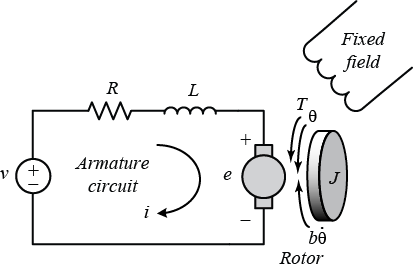
\includegraphics[width=0.9\columnwidth]{image63}
            \end{center}

        \end{column}
    \end{columns}

\[
    \theta(s) = \frac{K}{s \cdot ( (J \cdot s + b) \cdot (L \cdot s+ R) + K^2)} \cdot V(s)
\]

\pause

Can differentiate this expression to get the transfer function for speed

\[
    \dot\theta(s) = \frac{K}{(J \cdot s + b) \cdot (L \cdot s + R) + K^2} \cdot V(s)
\]


\end{frame}

%%%%%%%%%%%%%%%%%%%%%%%%%%%%%%%%%%%%%%%%%%%%%%%%%%%%%%%%%%%%%%%%%%
\section{Brushless DC motors}

{\fullbackground[scale=0.9,page=2]{ian-brushless-dc-motors.pdf}
\begin{frame}{Problems of mechanical commutation}

%Can get potential difference across commutator segments
%
%\begin{itemize}
%
%\item Can get potential difference across commutator segments
%\item Commutation shorts out the commutator segments
%\item Arcing and sparkling at the brushes
%\item Brushless electronic switching solves this issue
%\end{itemize}

\end{frame}
}

{\fullbackground[scale=0.9,page=3]{ian-brushless-dc-motors.pdf}
\begin{frame}{Brushless DC Motor}

%This motor type looks like DC brushed motor turned inside out!
%
%\begin{itemize}
%
%\item This motor type looks like DC brushed motor turned inside out!
%\item In an EC (brushless) motor, commutation is performed electronically to
%  eliminate brushes
%\item The stator generally consists of several coils
%\item Current flow in the stator coils creates magnetic field
%\item This forces the permanent magnet rotor turn
%\item The rotor can be forced to rotate continuously by switching on current
%  in the stator coils in the appreciate sequence thereby generating a
%  sequenced magnetic field
%\item All brushless motors require a controller to work that must perform
%  the commutation operation
%\end{itemize}

\end{frame}
}

{\fullbackground[scale=0.9]{image81}
\begin{frame}{Typical brushless motor}

\end{frame}
}


{\fullbackground[scale=0.9,page=5]{ian-brushless-dc-motors.pdf}
\begin{frame}{How do brushless motors work?}

%\begin{itemize}
%\item Electronic commutation is used to switch current in the stator could
%  so that the rotor is forced to rotate
%\item There is often a control magnet is in line with the poles of the large
%  magnet in the motor to identify rotor angle so that the controller can
%  switch current into the appropriate coils
%\item As it turns Hall sensors are stimulated by the magnetic flux.
%\item The Hall sensors are used to tell the controller what the orientation
%  is of the magnet with respect to the three winding phases.
%\item Current in the stator coils is turned on and off in sequence creating
%  motion from pole to pole.
%\end{itemize}

\end{frame}
}

{\fullbackground[scale=0.9,page=21]{../part1/figs/ian-sensors.pdf}
    \begin{frame}{Electronic commutation systems}
    \note {
In this third part of the presentation we would like to understand the electronic commutation.
There are different systems. maxon uses the following three :

- Block commutation with or without Hall sensors
- Sinusoidal commutation.

As you can see the different maxon controller families perform different commutation types.

Common to all these systems is that they should apply the current in a way, that the generated torque is as high as possible. As we have learned this is achieved by a perpendicular orientation of the magnetic fields of permanent magnet and winding. We have seen as well that we need to know the orientation of the permanent magnet to achieve this.

We start with block commutation with Hall sensor position feedback. That's the standard commutation type. Once we have understood this the two other commutation schemes are easily derived from it.
    }
    \end{frame}
}

{\fullbackground[scale=0.9,page=22]{../part1/figs/ian-sensors.pdf}
    \begin{frame}{Block commutation}

\note{
First we have to look at the Hall sensor feedback signals. Again we do this
based on the simplest design, the slotless maxon EC motor with 1 pole pair.

In the back of the motor there are three Hall sensor mounted on the PCB at an
angle of 120°. The Hall sensor detect the magnetic poles of the control magnet
which is mounted on the shaft. The control magnet exhibits the same two
magnetic poles in the same orientation as the power magnet. (Basically the Hall
sensors could monitor the power magnet directly but the control magnet offers
two advantages: The magnetic transitions between north and south pole are more
precisely defined. And an angular misalignment and tolerances between the
relative position of winding and Hall sensors can be adjusted.)

The digital Hall sensors used probe the direction of the magnetic field. They
generates a high output signal (5V) if the north pole of the control magnet is
close to them. A south pole produces a low level (Gnd).

The actual position of the control magnet in the diagram generates the
following signals:

- The blue Hall sensor sees the north pole. Thus the signal output level is
high and will remain high for the next 120°.
- The green Hall sensor is close to the south pole. The output level is low for
the next 60°. Then the north pole approaches and the output signal will switch
to a high state.
- The red Hall sensor has just switched from high to low where the signal level
will stay for the next half a turn.

The combination of the three Hall sensor signals is unique for each 60° of
rotation. Looking at these signals allows to know the rotor position within
60°. That exactly what we need for commutation. Remember there were 6 different
ways of current flow through the motor at a commutation angle of 60°.

The next slide shows how the complete block commutation system works.
}
    \end{frame}
}

{\fullbackground[scale=0.9,page=23]{../part1/figs/ian-sensors.pdf}
    \begin{frame}{Components of an EC drive system}
\note{
Let's first look at an EC drive system in general.

The three phases of the EC motor cannot be connected directly to a DC power
supply. The voltage needs to be switched in a sequence. This is done by the
electronic commutation. For the correct switching the electronics needs rotor
position information from the motor. This information is usually provided by
the Hall sensors.

An EC motor cannot operate on its own: It's always the combination of motor and
electronics commutation that makes the full drive.


For more sophisticated commutation and precise motor control, e.g. at very low
speeds, the use of an encoder feedback might be necessary. Often the
electronics not only performs the commutation but at the same time can be used
to control speed or position.
}
    \end{frame}
}


{\fullbackground[scale=0.9,page=6]{ian-brushless-dc-motors.pdf}
\begin{frame}{Block commutation}

%\begin{itemize}
%\item
%\end{itemize}
%
%\_
%
%HS3
%
%HS1
%
%HS2
%
%controller
%
%power stage
%
%(MOSFET)
%
%phase 1
%
%phase 2
%
%phase 3
%
%EC motor
%
%(magnet, winding, sensor)
%
%rotor position feedback
%
%commutation
%
%logics
%
    \note{

\textbf{On the right} we have a schematic \textbf{cross section of a
maxon EC motor} with 2 pole permanent magnet in the center, the three
phase winding and the three Hall sensors placed at 120°. For simplicity
we assume the Hall sensors to probe the power magnet directly.

\textbf{On the left} we have the \textbf{commutation electronics} which
is fed with a DC supply voltage. There is a power bridge made of 6
MOSFETs. Three of them are needed to contact the motor phases to the
positive supply voltage. The lower three MOSFETs make the contact to the
supply ground. The power bridge is controlled by a commutation logic
that evaluates the Hall sensor signals and, accordingly, switches the
power on the three motor phases.

\textbf{Comments on the animation:}

In this starting position the Hall sensors give the following signal:
HS1 has just switched to a high state, HS2 is low and HS3 is high.

The commutation logic knows that for this signal combination and
clockwise motor rotation the current must flow from phase 1 to 2 and
powers the respective two MOSFETs.

The winding produces a magnetic field and the magnetic rotor tries to
align.

After 60° the HS3 starts seeing the south pole. Its output switches to
low and the commutation logic switches the current from phase 1 to 3.
The field of the winding advances by 60° and the rotor continues to
rotate.

Again after 60° the Hall sensor pattern changes, HS2 switches to a high
output level. Accordingly the electronics commutates the current to flow
from phase 2 to 3. Again the field of the winding advances by another
60° and the rotor continues.

And so on \ldots{} . After 6 commutation intervals we are back at the
initial configuration and the rotor has accomplished one turn.

}

\end{frame}

}

{\fullbackground[scale=0.9,page=7]{ian-brushless-dc-motors.pdf}
\begin{frame}{Brushless motor for RC aircraft}

\end{frame}
}

{\fullbackground[scale=0.9,page=8]{ian-brushless-dc-motors.pdf}
\begin{frame}{Maxon EC brushless motor}

%Permanent magnet
%
%Special Winding
%
%Rotating part -- permanent magnet
%
%Hall sensors
%
%Control Magnet
%
%Case / Magnetic
%
%return

\end{frame}

}

{\fullbackground[scale=0.9,page=9]{ian-brushless-dc-motors.pdf}
\begin{frame}{Maxon EC flat brushless motor}

%Multi pole motor
%
%Flat design gives more torque as the flux is acting further from the
%centre of rotation

\end{frame}

}

{\fullbackground[scale=0.9,page=10]{ian-brushless-dc-motors.pdf}
\begin{frame}{Advantages and disadvantages of EC}

%\textbf{Brushed DC motors}
%
%\begin{itemize}
%
%\item Mechanical commutation
%\item Need periodic brush maintenance
%\item Power losses in brushes
%\item Sparking
%\item Can have noisy operation
%\item Linear torque characteristic at lower
%\item Change direction by changing voltage polarity
%\item Controller not always needed
%\end{itemize}
%
%\textbf{EC motors}
%
%\begin{itemize}
%
%\item Electronic commutation
%\item Low or no maintenance
%\item Less power loss
%\item No sparking
%\item Quieter operation
%\item More linear torque characteristic
%\item Change direction by changing switching sequence
%\item Always needs drive controller circuitry
%\item Requires sensors
%\item Higher reliability \& efficiency
%\item Stator on outside -- better for heat dissipation
%\item Longer life
%\item More expensive
%\end{itemize}

\end{frame}
}

%\section{Some other motors}
%
%\begin{frame}{Wound field motors}
%
%\begin{itemize}
%
%\item What happens if we apply AC to a permanent magnet DC motor?
%\end{itemize}
%
%\end{frame}
%
%\begin{frame}{Motor with stator winding}
%
%\end{frame}
%
%\begin{frame}{Shunt motor}
%
%\begin{itemize}
%\item Like DC motor but with electromagnet to generate static field
%\item Armature and field windings are connected in parallel
%\item Separate current through stator and armature
%\item Low Starting Torque
%\item Good Speed Regulation
%\item Used for fixed speed applications, windscreen wipers, fans
%\end{itemize}
%
%\end{frame}
%
%\begin{frame}{Shunt motor}
%
%Consider motor behavior under load:
%
%\begin{itemize}
%
%\item On application of load speed will reduce
%\item But this reduced armature EMF
%\item Therefore armature current rises
%\item Therefore torque increases
%\item So speed increases too
%\item Therefore system can do some self regulation of speed
%\item Much like permanent magnet DC motor!
%\end{itemize}
%
%\end{frame}
%
%\begin{frame}{Series motor}
%
%\begin{itemize}
%
%\item Armature and field windings are connected in series
%\item Same current goes through both
%\item High Starting Torque
%\item As the speed builds up so does the back EMF, reducing the current,
%  which causes a reduction in torque
%\item Poor Speed Regulation
%\item Used for starting heavy, industrial, high torque loads such as cranes,
%  hoists, elevators, trolleys and conveyors
%\item Cannot operate safely in an unloaded condition
%\end{itemize}
%
%\end{frame}
%
%\begin{frame}{Universal Motors}
%
%\begin{itemize}
%
%\item Series motor
%\item Uses field coils and not permanent magnets
%\item AC and DC operation
%\item As current direction changes it changes field direction on stator
%  field and also armature
%\item So always rotates in same direction independent of applied current
%  direction
%\end{itemize}
%
%\end{frame}



%%%%%%%%%%%%%%%%%%%%%%%%%%%%%%%%%%%%%%%%%%%%%%%%%%%%%%%%
%%%%%%%%%%%%%%%%%%%%%%%%%%%%%%%%%%%%%%%%%%%%%%%%%%%%%%%%
\miniframesoff
\begin{frame}{}
    \begin{center}
        \Large
        That's all, folks!\\[2em]

        \normalsize
        \textbf{Questions}:\\
        Portland Square B316 or \url{severin.lemaignan@plymouth.ac.uk} \\[1em]

        \textbf{Slides}:\\
        \href{https://github.com/severin-lemaignan/module-introduction-sensors-actuators}{\small
        github.com/severin-lemaignan/module-introduction-sensors-actuators} \\

        ...or the DLE!


    \end{center}
\end{frame}




\end{document}
